\documentclass[25pt,a0paper,portrait]{tikzposter}
\usepackage[utf8]{inputenc}
\usepackage{xcolor}
\usepackage{graphicx}
\usepackage{tikz}

\makeatletter
\def\TP@titlegraphictotitledistance{-6cm}
\settitle{
	\centering
	\vbox{
		\@titlegraphic \\ [\TP@titlegraphictotitledistance]
		\centering
		\color{titlefgcolor}
		{\bfseries \Huge \sc \@title \par}
		\vspace*{1em}
		{\huge \@author \par}
	}
}
\makeatother

\setlength{\columnsep}{1.5cm}

\title{License Plate Detection System}
\author{Gautam, Sidhanth, Shubhankar}
\titlegraphic{\raisebox{0.7cm}{%
	
\includegraphics[height=6.8cm]{images/logo_hs_technik}}
	\hfill
	\vspace{-0.45cm}
	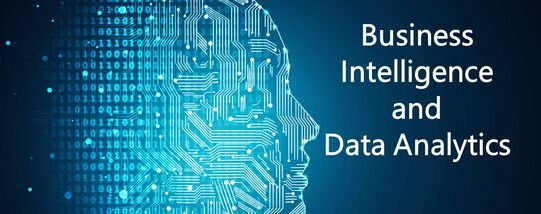
\includegraphics[height=7.8cm]{images/BIDA}
}

\usetheme{Desert}

\begin{document}
	
	\maketitle
	
		\begin{columns}
			
		% Left column: Problem Description + Challenges
		\column{0.5}
		{
			\colorlet{blocktitlebgcolor}{blue}
			\block{Problem Description}
			{
					Efficient vehicle handling at high-throughput gates (airport drop-off / parking) needs fast and reliable identification without manual checks. This project implements an \textbf{edge-first} License Plate Detection System on the \textbf{NVIDIA Jetson Nano}, using a single USB camera and on-device inference to support gate-level decisions.\newline

					\begin{itemize}
						\item \textbf{Use case:} recognize vehicles at entry/exit lanes, track their visit duration, and support a billing / time-limit decision at the gate.
						\item \textbf{Design goals:} low latency, continuous operation, and on-device persistence so the system can recover cleanly after restarts.
						\item \textbf{End-to-end pipeline (on device):}
						\begin{itemize}
							\item Camera capture \(\rightarrow\) YOLOv8 plate detection (TensorRT) \(\rightarrow\) crop + preprocessing \(\rightarrow\) EasyOCR (CPU) \(\rightarrow\) validation \(\rightarrow\) database logging.
							\item A cooldown/stability window reduces repeated OCR on near-identical frames while still reacting quickly to new vehicles.
						\end{itemize}
						\item \textbf{Recorded data:} plate string with \textbf{first-seen} and \textbf{last-seen} timestamps stored in a local \textbf{SQLite} database (\texttt{parking.db}) for persistence.
						\item \textbf{Billing concept:} dwell time is derived from \texttt{last\_seen\_ts - entry\_ts}; deployment parameters (e.g., tariff, grace window) are configured as runtime constants.
						\item \textbf{Outputs:} live annotated video stream and a local web dashboard showing recent plates, timestamps, and computed fee.
					\end{itemize}
					
				}
				
				\block{Challenges}
				{
				Deploying license plate recognition on a low-power edge device introduces practical constraints beyond model accuracy:\newline
				
				\begin{itemize}
					\item \textbf{Compute + memory limits (edge hardware):} the Jetson Nano has 4\,GB unified memory shared between CPU and GPU. This restricts model size, limits parallel workloads, and requires careful balancing between detection and OCR.
					\item \textbf{Storage constraints (production module):} internal storage is limited (16\,GB eMMC) and our deployment does \textbf{not} use an SD card; models, logs, and the database must be placed on an external SSD.
					\item \textbf{Runtime robustness:} long continuous runs can trigger memory pressure and performance throttling; stable operation requires careful resource management (swap usage, conservative pipelines).
					\item \textbf{Legacy software ecosystem:} JetPack 4.6 (Ubuntu 18.04 / Python 3.6) constrains library versions and increases integration effort when using modern ML tooling.
					\item \textbf{Real-world imaging conditions:} variable lighting, glare, dirty plates, motion blur, and oblique viewing angles reduce OCR quality even when plate detection is correct.
					\item \textbf{OCR ambiguity + validation:} similar-looking characters and perspective distortion require allowlists and format validation (German plate constraints) to reduce false reads.
					\item \textbf{Timing in real time:} OCR is computationally expensive; the runtime must avoid repeated OCR on every frame (cooldown/stability) while still reacting quickly to new vehicles.
				\end{itemize}
				
					
				}
			}
		
		% Right column: Sales Dashboard + Solutions + Results stacked
		\column{0.5}
		{
			\colorlet{blocktitlebgcolor}{blue}
			\block{System Illustration}
			{
			\begin{center}
				\vspace{-0.3cm}
				\includegraphics[width=0.95\linewidth,keepaspectratio]{images/JetsonNanoPoster}
			\end{center}
			}
			
			\block{Solutions}
			{
			
			We combined hardware-aware deployment, optimized inference, and practical validation logic to achieve real-time operation on the Jetson Nano:
			
			\begin{itemize}
				\item \textbf{Hardware-aware deployment}
				\begin{itemize}
					\item Store runtime artefacts (TensorRT engine + database) on an \textbf{external SSD} mounted at \texttt{/media/myssd}.
					\item Use swap on SSD to reduce out-of-memory failures during long runs.
				\end{itemize}
				
				\item \textbf{Real-time detection on GPU}
				\begin{itemize}
					\item Deploy the detector as a \textbf{TensorRT} engine (\texttt{best.engine}) for accelerated inference.
					\item Use a lightweight model variant suitable for stable edge performance.
				\end{itemize}
				
				\item \textbf{OCR + validation on CPU}
				\begin{itemize}
					\item Run \textbf{EasyOCR} in CPU mode and preprocess plate crops (resize + thresholding) for improved readability.
					\item Apply an allowlist and German-format validation (city-prefix handling + numeric suffix rules) to reduce false reads.
				\end{itemize}
				
				\item \textbf{Persistence + local UI}
				\begin{itemize}
					\item Log visits to a local SQLite database (\texttt{parking.db}) with \texttt{entry\_ts} and \texttt{last\_seen\_ts}.
					\item Provide a local Flask dashboard (live stream + billing table) for on-site monitoring and reporting.
				\end{itemize}
			\end{itemize}
			
			}
			
			\block{Results}
			{
			The system runs end-to-end on the Jetson Nano and produces actionable, real-time outputs suitable for continuous edge operation:
			
			\begin{itemize}
				\item \textbf{Real-time performance:} stable detection throughput of \(\approx\)13--15 FPS using TensorRT acceleration.
				\item \textbf{End-to-end workflow:} camera capture \(\rightarrow\) plate detection \(\rightarrow\) OCR \(\rightarrow\) validation \(\rightarrow\) database logging \(\rightarrow\) dashboard display.
				\item \textbf{Operational output:} the dashboard lists recognized plates with timestamps and a computed dwell-time fee from stored visit data.
				\item \textbf{Edge-first operation:} processing and logging are performed locally; only lightweight visit metadata is stored for persistence.
				\item \textbf{Deployment:} Jetson Nano (4\,GB) with external SSD storage for runtime artefacts.
			\end{itemize}
			}
		}
		
	\end{columns}
	
\end{document}
